\graphicspath{ {./Figure/Figure10/}}
\begin{figure}
  \centering
	
  \hspace*{\fill}
  \subfigure[]{\label{subfig:8a}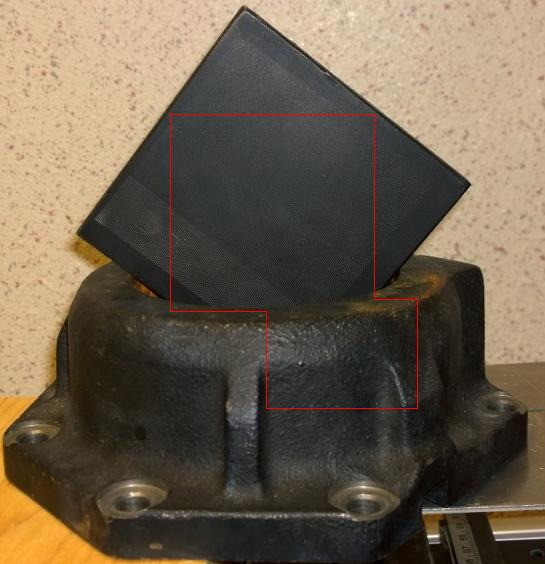
\includegraphics[width=0.3\linewidth]{fig8a.png}}\hfill
  \subfigure[]{\label{subfig:8b}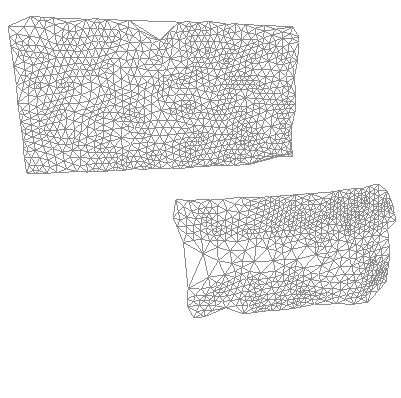
\includegraphics[width=0.3\linewidth]{fig8b.png}} 
	\hspace*{\fill} \\ \hspace*{\fill}
  \subfigure[]{\label{subfig:8c}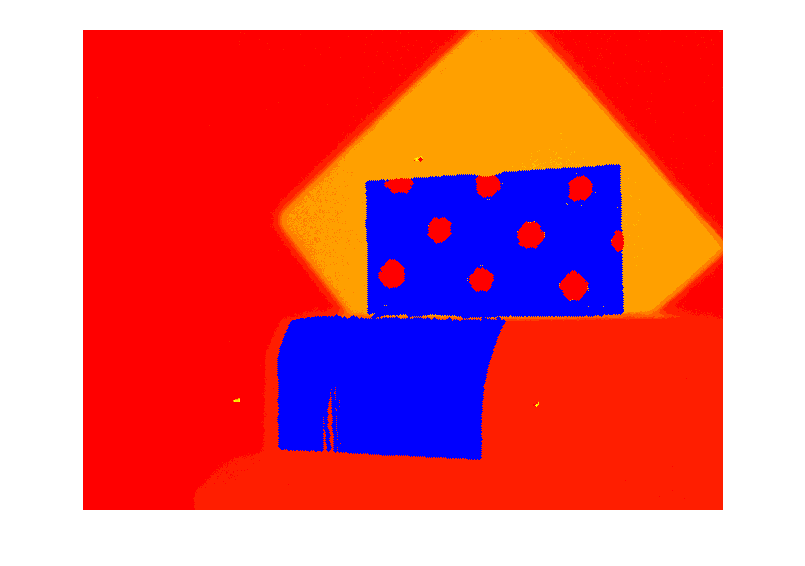
\includegraphics[width=0.3\linewidth]{fig8c.png}} \hfill
  \subfigure[]{\label{subfig:8d}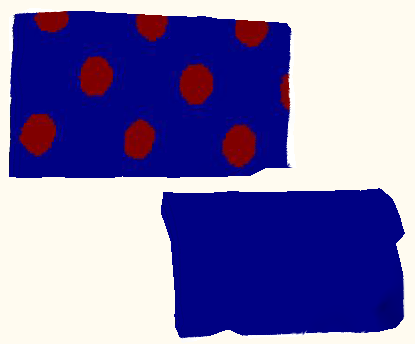
\includegraphics[width=0.3\linewidth]{fig8d.png}}
  \hspace*{\fill}
	
	\caption{(a) The specimen - (b) 3D mesh - (c) Corresponding detection map - (d) 3D mapping.}
  \label{fig:8}
\end{figure}
